The amazon dataset was the first mandatory dataset, were we accomplished a score of 72.8\% on kaggle competition. Especially the high dimensionality was the challenge of this dataset.

\subsection{Characteristics}

\begin{itemize}
\item No missing values
\item 50 different target classes
\item Only rational data
\item 10 000 attributes
\item 750 samples
\end{itemize}

With its 10 000 attributes it is high dimensional.
Therefore Feature Selection is important, but features can not be interpreted by hand, because there are too many of them.
In order to find good features algorithms from scikit were used, as described in section \ref{fig:amazon-feature-selection}.

\subsection{Characteristics of Target value}
The target classes are the different authors of the reviews.
There are 50 different authors and even though the dataset has a lot of samples, there are only a few samples per class.
This is shown in Figure \ref{fig:amazon-target}. With a minimum of 8 samples written by CFH and a maximum of 21 samples written by Chell. 
On the other hand 10 000 attributes for each sample might be sufficient for a good and useful classification result.

\image{amazon/plots/target.png}{Histogram of the target values}{\label{fig:amazon-target}}

% \begin{figure}[H]
%   \begin{center}
%     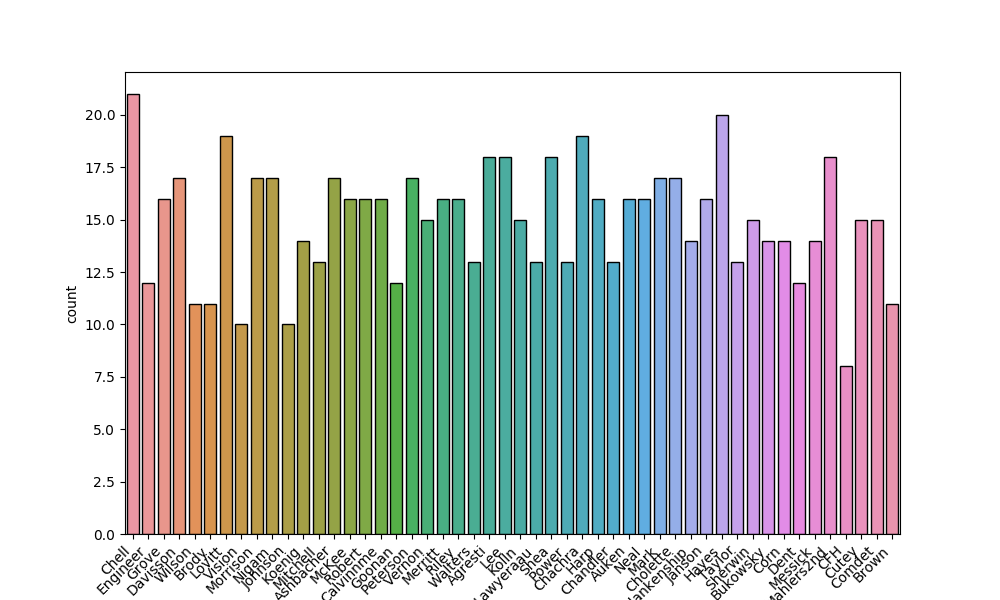
\includegraphics[width=\linewidth]{amazon/plots/target.png}
%     \caption{Histogram of the target values}
%     \label{fig:amazon-target}
%   \end{center}
% \end{figure}


\subsection{Feature selection}
\label{amazon-feature-selection}
Feature selection improves results and reduces the runtime a lot. It was not feasible to train the multi layer perceptron without feature selection, because producing a representative result with cross validation would have taken over 10 minutes to complete. Thus, a comparison without feature selection was not done. Selecting specific attributes results in a general improvement of 20\%-40\% depending on the classifier and the amount of chosen attributes. 

Features were selected by SelectKBest and recursive feature elimination and cross-validated selection of the best numbers of features.
SelectKBest performs a ${\chi}^2$ test on the samples to retrieve the best features.
As seen in Figure \ref{fig:amazon-feature-selection} at least 1000 features should be used to cross the 55\% mark, however no difference in performance could be detected between 1000 and 4000 selected features.

\image{amazon/plots/rf_feature_selection.png}{recursive feature selection with random forest tree}{\label{fig:amazon-feature-selection}}

% \begin{figure}[H]
%   \begin{center}
%     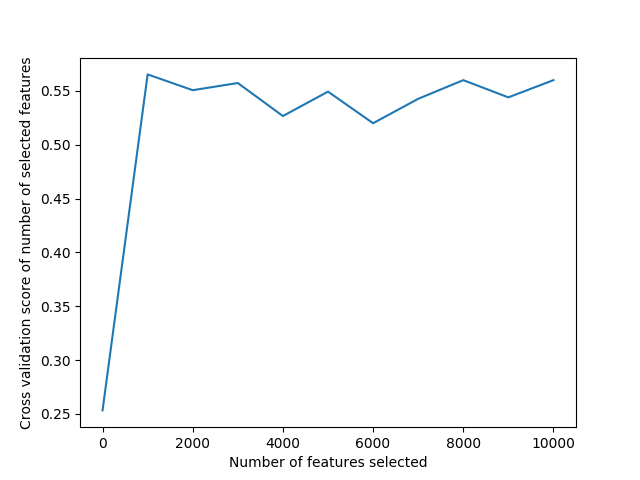
\includegraphics[height=7cm]{amazon/plots/rf_feature_selection.png}
%     \caption{Comparison of different metrics}
%     \label{fig:amazon-feature-selection}
%   \end{center}
% \end{figure}

\subsection{K Nearest Neighbors Classifier}

For K Nearest Neighbours a Grid Search with cross validation was used. The euclidean, chebyshev, manhattan, manhattan and a \textit{k} between 1 and 60 were tested. 
The best \textit{k} for KNN without preprocessing and all attributes was 10.
The best \textit{k} for KNN with preprocessing and features selected by recursive feature selection was 15.
K Nearest Neighbours Classifier worked best with weights set to distance, so that the importance of the k neighbours are weighted by their distances to other samples.
This increased results by about 5\%. As seen in Figure \ref{fig:amazon-knn-metric-comparison} the manhattan metric worked best.
The best performance of KNN was 44.13\% which is poor in comparison to the Random Forest Classifier or the Multi-Layer Perceptron.
This is probably due to the small sample size in comparison to the target class size.
However, it evaluates much faster, and therefore a first impressions could be derived quicker, when comparing to other techniques, which is no surprise since KNN is a lazy learner.

\image{amazon/plots/knn_metrics.png}{Comparison of knn metrics}{\label{fig:amazon-knn-metric-comparison}}
% \begin{figure}[H]
%   \begin{center}
%     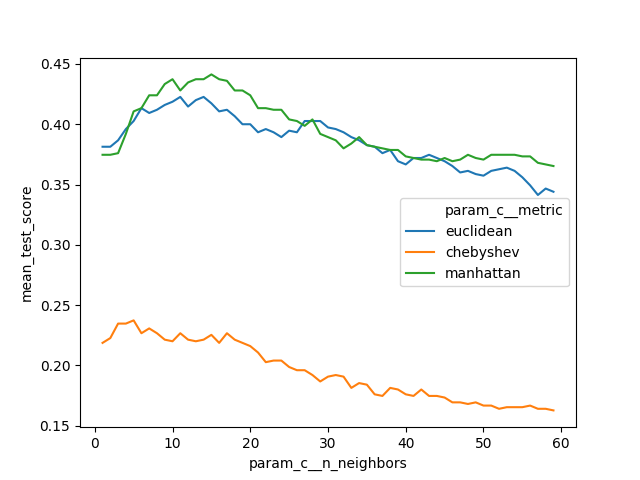
\includegraphics[width=\linewidth]{amazon/plots/knn_metrics.png}
%     \caption{Comparison of different metrics}
%     \label{fig:amazon-knn-metric-comparison}
%   \end{center}
% \end{figure}

Preprocessing with MinMax scalar improved results by around 5\%, as seen in Figure \ref{fig:amazon-knn-comparison}.
Scaling with mean and variance lead to better results as well, but it was not as good as the MinMax scaler.

\image{amazon/plots/knn_comparison.png}{Comparison of the best estimators with preprocessing and without preprocessing}{\label{fig:amazon-knn-comparison}}

% \begin{figure}[H]
%   \begin{center}
%     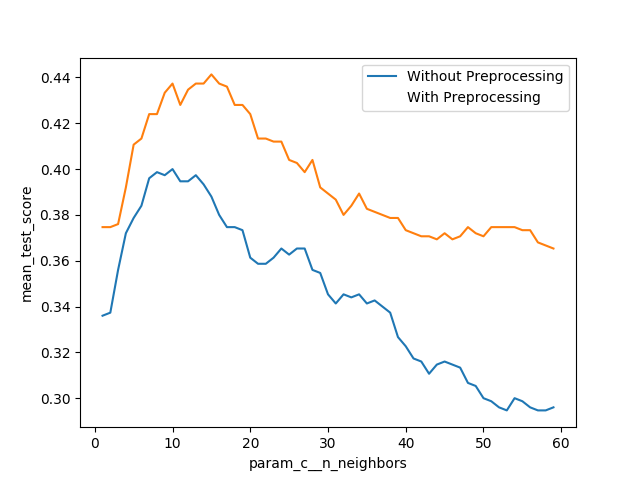
\includegraphics[width=\linewidth]{amazon/plots/knn_comparison.png}
%     \caption{Comparison of the best estimators with preprocessing and without preprocessing}
%     \label{fig:amazon-knn-comparison}
%   \end{center}
% \end{figure}


\subsection{Random Forest Classifier}

As previously described a grid search with cross validation was used to find the best parameters for the amazon dataset.
However trying and varying all parameters would explode the search space, hence a random search with cross validation was used to approximate features first.
Then the more specific grid search with a smaller search space based on the obtained results, was performed.
The best features of Figure \ref{fig:amazon-feature-selection} were used to improve the results even more. 
As seen in Figure \ref{fig:amazon-rf-comparison}, low maximum features yielded to good results, because of the high dimensionality.
With 34 estimators and 30\% max features, a score of 60\% was accomplished which is almost as good as the multi layer perceptron.
However it took significantly longer to fit and evaluate than KNN.

\image{amazon/plots/rf_comparison.png}{Comparison of random forest parameters}{\label{fig:amazon-rf-comparison}}

% \begin{figure}[H]
%   \begin{center}
%     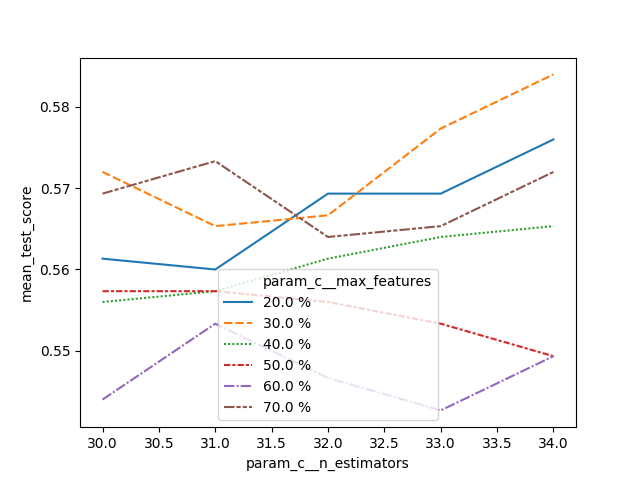
\includegraphics[width=\linewidth]{amazon/plots/rf_comparison.png}
%     \caption{Comparison of the best estimators with preprocessing and without preprocessing}
%     \label{fig:amazon-rf-comparison}
%   \end{center}
% \end{figure}

\subsection{Multi-Layer Perceptron Classifier}

For MLP a grid search with a small search space was used, because testing out different to many hyperparameters is not feasible, because it takes a lot of time and computation power.`
As shown in Figure \ref{fig:amazon-mlp-comparison} choosing different activation functions does hardly make any difference.
A score of 72.8\% in accuracy was obtained in the kaggle competition by  selecting 2000 features with the ${\chi}^2$ tests, using relu as activation function, having one hidden layer with 100 neurons and setting max iterations on 4000.

\image{amazon/plots/mlp_comparison.png}{Comparison of mlp parameters}{\label{fig:amazon-mlp-comparison}}

% \begin{figure}[H]
%   \begin{center}
%     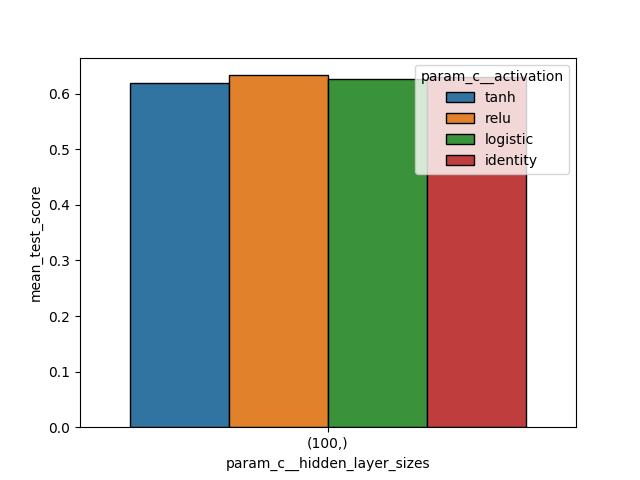
\includegraphics[width=\linewidth]{amazon/plots/mlp_comparison.png}
%     \caption{Comparison of the best estimators with preprocessing and without preprocessing}
%     \label{fig:mlp-comparison}
%   \end{center}
% \end{figure}

\subsection{Conclusion}

Scaling and feature selection improve results for most classifiers quite a bit. While scaling does not affect the random forest classifier, it has a huge impact on both, k nearest neighbours and the multi layer perceptron. Feature selection is important for all classifiers. Support Vector machines were tried out as well, because they are suited for high dimensional data, but only resulted in a maximum score of 63.46\%

\begin{table}[ht]
\begin{center}
\begin{tabular}{|l|l|l|}
\hline
                       & Preprocessing & No-Preprocessing \\ \hline
KNeighborsClassifier   & 0.4413        & 0.4000           \\ \hline
RandomForestClassifier & 0.6026        & 0.5840           \\ \hline
MLPClassifier          & 0.6746        & 0.6133           \\ \hline
\end{tabular}
\caption{Comparison of accuracy of different techniques with- and without preprocessing}
\end{center}
\end{table}

Holdout obviously yields different results than cross validation. Although cross validation takes a lot of time for parameter optimization, it generally give more accurate average predictions, whereas hold out is quicker but might not be as accurate. Accuracy between holdout and cross validation differs up to 5\_%.

\begin{table}[ht]
\begin{center}
\begin{tabular}{|l|l|l|}
\hline
                       & Holdout & Cross Validation \\ \hline
KNeighborsClassifier   & 0.4066  & 0.4413           \\ \hline
RandomForestClassifier & 0.5333  & 0.5946           \\ \hline
MLPClassifier          & 0.6133  & 0.6746           \\ \hline
\end{tabular}
\caption{Comparision of accuracy of holdout versus cross-validation}
\end{center}
\end{table}

Accuracy is the most useful measurement for the amazon dataset, because the most interesting goal is to find out which review is written by which author.
The runtime is the average runtime it took to fit the train data for each of the 10 folds. The MLP classifier was faster than the random forest tree classifier, because it had a very basic structure and less max iterations in order to run faster and stop it from overfitting.
Other than that knn was the fastest, because, as already mentioned, it is a lazy learner. As expected MLP had the highest accuracy.

\begin{table}[ht]
\begin{center}
\begin{tabular}{|l|l|l|l|l|l|}
\hline
                       & Accuracy & Precision & Recall & F1     & Runtime (sec) \\ \hline
KNeighborsClassifier   & 0.4333   & 0.3847    & 0.4356 & 0.3805 & 30.987        \\ \hline
RandomForestClassifier & 0.5946   & 0.5400    & 0.5893 & 0.5393 & 481.152       \\ \hline
MLPClassifier          & 0.7000   & 0.6611    & 0.6940 & 0.6534 & 96.535        \\ \hline
\end{tabular}
\caption{Comparision of different performance metrics and runtimes}
\end{center}
\end{table}

